\chapter{GUI}

The Software consists of three main parts:
\begin{enumerate}
	\item The GUI part is responsible for graphical representation of the Software and interaction with the user. The GUI part is a glue that connects all other parts together. It is based on PySide6 library which is a Python port of the famous QT library.

	\item The driver part is responsible for communications with the reflectometer. It provide the high-level interface functions such as `connect', `get parameters', `set parameters', 'run measurements' and so on. When one of these functions is called, this part translates it to the appropriate command codes of the Reflectometer (see AQ7270 Series OTDR
	Communication Interface).
	

	\item Plugins are responsible for data processing and visualisation. When the new reflectogram is obtained, it is sent to all active plugins. 
\end{enumerate}


\section{Control buttons}

\begin{itemize}
	\item Single measurement
	\item Monitoring
	\item Autosave
\end{itemize}


\section{Plugins}

\subsection{Averager}

	The averager plugin collects reflectograms, calculates an average and estimates the deviation of the current reflectogram from the average.
	
	We use the following designations.
	\begin{itemize}
		\item Vector $y$ is the recently measured reflectogram (the current reflectogram).
		\item $M$ is the total number of points (samples) in each reflectogram. 
		\item $j$ is used to enumerate points, $j = 1, \ldots, M$. 
		\item $x_j$ is the distance to $j$-th point.
		\item The graphical representation of reflectogram $y$ can be considered as the set of points
		\begin{equation*}
			\left\{(x_1, y_1), (x_2, y_2), \dots, (x_M, y_M)\right\}.
		\end{equation*}
		\item Matrix $Y$ contains all previously measured reflectograms concatenated horizontally as columns. In other words, $Y_{ji}$ is the $j$-th point of $i$-th reflectogram. The size of $Y$ is $M \times N$, where $N$ is the number of reflectograms stored in $Y$.
	\end{itemize}		
	
	The following steps are made when the new reflectogram is obtained.
	First, we calculate the \textbf{mean reflectogram} as 
	\begin{equation}
		\mean{y}_j = \frac{1}{N}\sum\limits_{i=1}^{N} y_{ji},
	\end{equation}
	and the unbiased sample variance as
	\begin{equation}
		\sigma_{j} = \sqrt{\frac{1}{N-1}\sum\limits_{i=1}^{N} \left(y_{ji} - \mean{y}_j\right)^2}.
	\end{equation}

	The \textbf{upper and lower bounds} are calculated as
	\begin{align}\label{eq:y_lower_upped_def}
		y^{lower}_{j} &= \mean{y}_j - n\sigma_{j}, \\
		y^{upper}_{j} &= \mean{y}_j + n\sigma_{j},
	\end{align}
	where $n$ is some number, usually $n$ is chosen from interval $\left[2, 5\right]$.
	
		
	The \textbf{violation level} is calculated as
	\begin{equation}
		V = \frac{1}{j_b - j_a + 1}\sum\limits_{j=j_a}^{j_b} \mathbf{I}\left\{y_{j} < y^{lower}_j \lor y_{j} > y^{upper}_j\right\},
	\end{equation}
	where indexes $j_a$ and $j_b$ define the segment of interest $\left[j_a, j_b\right]$. These indexes are calculated using the following formulas:
	\begin{align}
		j_a &= \max \left\{j: x_j < a\right\}, \\
		j_b &= \min \left\{j: x_j > b\right\},
	\end{align}
	where $a$ and $b$ are the left and right boundaries of the segment, expressed in metres.
	
	Finally, we compare $V$ with threshold $\Theta$. There are two cases.
	\begin{enumerate}
		\item If $V \leq \Theta$, then the current reflectogram is appended to $Y$. If the number of columns in $Y$ becomes greater than some predefined value, the most oldest columns are removed.
		\item If $V > \Theta$, the alarm is turned on. In this case, the current reflectogram $y$ is not appended to the end of $Y$.
	\end{enumerate} 
			
	
The parameters selection window is shown in Fig. \ref{fig:AverParamsWnd}. The parameters have the following sense.
\begin{itemize}
	\item `Aver count' is the maximum number of reflectograms stored by the plugin. In other words, it is the maximum number of columns in $Y$.
	\item `xmin, m' is the left boundary of the segment of interest, in meters. If it equals to None, then it means that xmin=0.
	\item `xmax, m' is the right boundary of the segment of interest, in meters. If it equals to None, then it means that xmax is selected to be equal to the actual number of samples, i.e. xmax = $M$. (corresponds to the right boundary of the reflectogram).
	\item `nsigma' corresponds to $n$ in eq. (\ref{eq:y_lower_upped_def}).
	\item `Violation threshold' corresponds to variable $\Theta$ defined above.
\end{itemize}
	
\begin{figure}[h]
	\begin{center}
		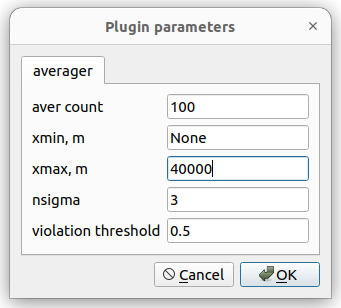
\includegraphics[width=6cm]{pictures/averager_parameters.png}
	\end{center}
	\caption{The parameters of the averager plugin}
	\label{fig:AverParamsWnd}
\end{figure}

\subsection{Final remarks}
\begin{itemize}
	\item If $N$ is low, the mean reflectogram is unreliable. Therefore, the averager plugin doesn't calculates the mean value, lower and upper boundaries if $N$ is less than 5. All new reflectograms are stored to $Y$. 
%	\item On initial phase, when all reflectograms are stored to $Y$, the averager plugin is vulnerable.
	\item In practice, reliable statistics can be obtained if $N$ is large (at least, $N > 100$). It should be guaranteed that there is no eyedropper on the initial phase.
\end{itemize}

\subsection{Plotters}
The averager plugin has two plotters to represent it state. First plotter draws the current reflectogram, mean reflectogram, and lower and upper boundaries in conventional axes. The vertical axis shows the signal level in dB, that is read directly from the device. 

The second plotter shows the deviation of the current reflectogram and lower and upper boundaries from the mean. The vertical axis is graduated in dB too, but shows the difference of the signal levels.


\begin{figure}
	\begin{subfigure}[b]{0.5\textwidth}
		\centering
		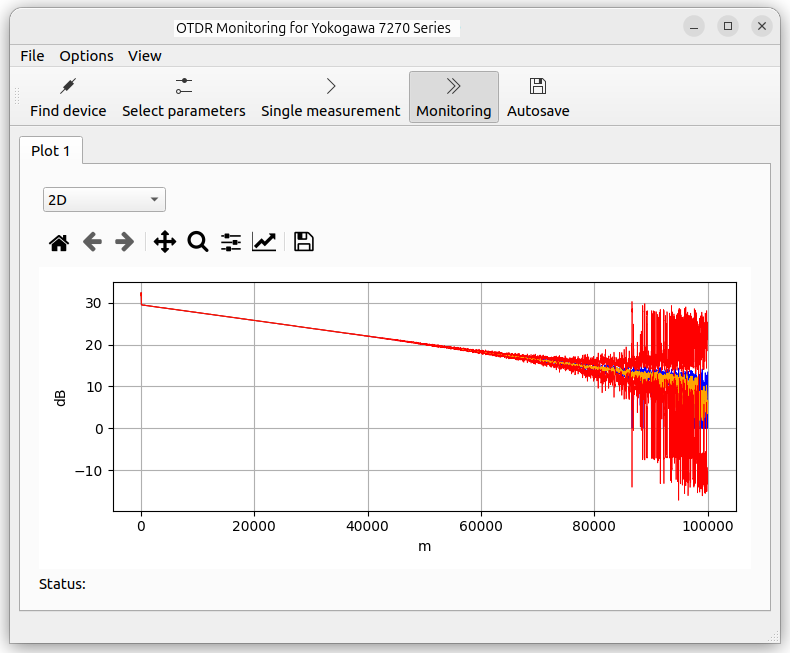
\includegraphics{pictures/averager2d.png}
		\caption{The default view of the reflectogram.}
	\end{subfigure}
	\hfill
	\begin{subfigure}[b]{0.5\textwidth}
		\centering
		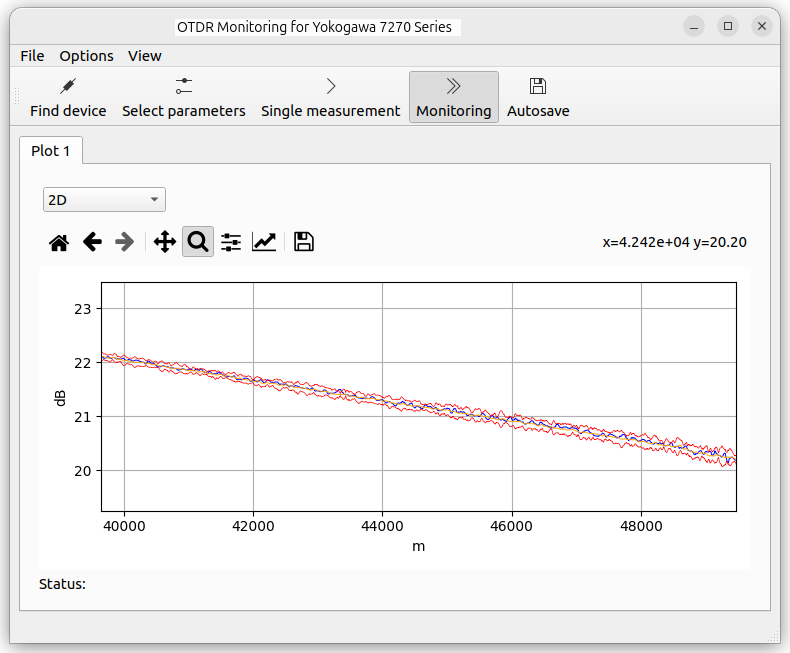
\includegraphics{pictures/averager2d_zoom.png}
		\caption{The magnified view.}
	\end{subfigure}

	\caption{The reflectogram in conventional axes. Red curves represent lower and upper boundaries. The blue curve is the current reflectogram. The orange curve is the mean reflectogram.}
\end{figure}


\begin{figure}
	\begin{subfigure}[b]{0.5\textwidth}
		\centering
		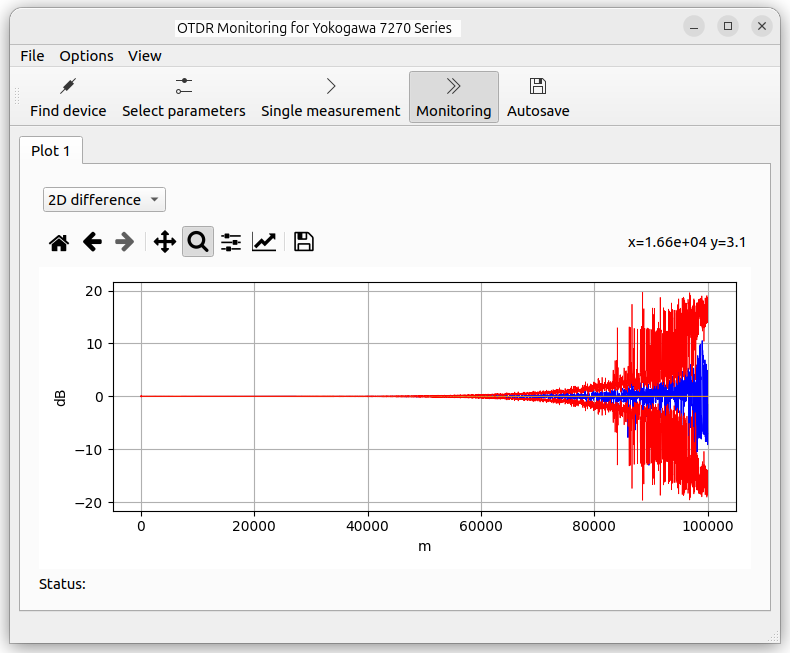
\includegraphics{pictures/averager2ddiff.png}
		\caption{The default view of the reflectogram.}
	\end{subfigure}
	\hfill
	\begin{subfigure}[b]{0.5\textwidth}
		\centering
		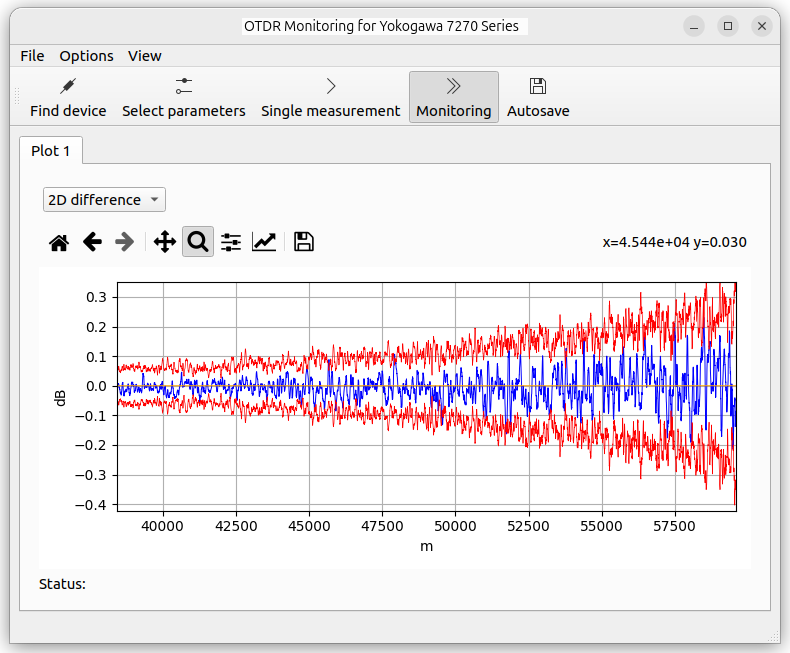
\includegraphics{pictures/averager2ddiff_zoom.png}
		\caption{The magnified view.}
	\end{subfigure}
	
	\caption{The deviation from the mean. As above, red curves are the lower and upper boundaries, and the blue curve is the current reflectogram. The orange horizontal line is $y = 0$.	}
\end{figure}
